\section{Definición de la tarea} \label{tarea}

En la siguiente tarea se solicita crear tres peticiones o query a un servidor desde una interfáz web. Estas peticiones deben ser de gran esfuerzo, es decir, se debe procesar una gran cantidad de datos desde la base de datos.\\

Posteriormente realizadas estas query se deben realizar 5 iteraciones para omptimizar estas solicitudes. Estas iteraciones buscan reducir los tiempos de espera del usuario que solicita la gran cantidad de datos a la base de datos.\\

Finalmente realizadas las iteraciones que buscan otpimizar las solicitudes. Se debe realizar una pruebas de carga con la herramienta Jmeter. Estas pruebas buscan estudiar el comportamiento de estas mismas consultas optimizadas pero suponiendo que varios usuarios accederán a ellas en un tiempo simultaneo. Cabe mencionar que las pruebas se deben realizar en un entorno "limpio", es decir, suponer que el dispositivo del usuario no se ve afectado por otros programas o por otros problemas de rendimiento. \\

\section{Consultas Básicas a la base de datos mediante una interfáz web}

En un comienzo se realizó una interfaz web, la cual cuenta con 3 botones, en donde cada botón al presionarlo genera una consulta a la base de datos \textbf{"employees"} como se muestra en la siguiente figura\ref{Figura}. 

\begin{figure}[htb]
	\label{Figura}
	\begin{center}
		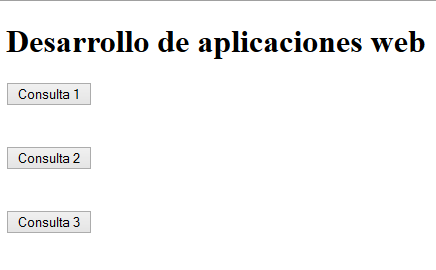
\includegraphics[scale=0.5]{imagenes/inicio.png}
	\end{center}
	\caption{Figura de la interfáz de inicio de la página web de consultas.}
\end{figure}
 
 
